\documentclass[a4paper]{article}

\usepackage[utf8]{inputenc}
\usepackage[portuguese]{babel}
\usepackage{a4wide}
\usepackage[pdftex]{hyperref}
\usepackage{graphicx}
\graphicspath{ {imagens/} } % path de imagens começa nesta pasta
\usepackage{wrapfig}
\usepackage{caption}
\usepackage{float}
\usepackage{amsmath}
\usepackage{subcaption}
\usepackage{tikz}
\usepackage{placeins}
\usetikzlibrary{patterns}

%%%%%%%%%%%%%%%%%% SQL STYLE %%%%%%%%%%%%%%%%
\usepackage{xcolor,listings}
\usepackage{textcomp}
\usepackage{color}

\definecolor{codegreen}{rgb}{0,0.6,0}
\definecolor{codegray}{rgb}{0.5,0.5,0.5}
\definecolor{codepurple}{HTML}{C42043}
\definecolor{backcolour}{HTML}{F2F2F2}
\definecolor{bookColor}{cmyk}{0,0,0,0.90}  
\color{bookColor}

\lstset{upquote=true}

\lstdefinestyle{mystyle}{   
    commentstyle=\color{codegreen},
    keywordstyle=\color{codepurple},
    numberstyle=\numberstyle,
    stringstyle=\color{codepurple},
    basicstyle=\footnotesize\ttfamily,
    breakatwhitespace=false,
    breaklines=true,
    captionpos=b,
    keepspaces=true,
    numbers=left,
    numbersep=10pt,
    showspaces=false,
    showstringspaces=false,
    showtabs=false,
}
\lstset{style=mystyle}

\newcommand\numberstyle[1]{%
    \footnotesize
    \color{codegray}%
    \ttfamily
    \ifnum#1<10 0\fi#1 |%
}
%%%%%%%%%%%%%%%%%%%%%%%%%%%%%%%%%%%%%%%%%%%%%%


% Fonte de jeito! Times New Roman <3
\usepackage{times}

\newcommand{\question}[1]{\textcolor{gray}{\textit{"#1"}}} % style para questões

\begin{document}

\begin{titlepage}
\begin{center}


\includegraphics[width=0.6\textwidth]{capa/logo.jpg}\\[.75cm]

\textsc{\LARGE Universidade do Minho}\\[0.7cm] % Name of your university/college
\textsc{\Large Departamento de Informática}\\[0.7cm] % Major heading such as course name
\textsc{\large Administração e Exploração de Base de Dados}\\[0.7cm] % Minor heading such as course title]

% Title
\rule{\linewidth}{0.5mm} \\[0.5cm]
{ \huge \bfseries Monitor de uma Base de Dados Oracle\\[0.5cm] }
\rule{\linewidth}{0.5mm}\\[0.7cm]

% Date
{\Large \today}\\[1cm] % Date, change the \today to a set date if you want to be precise

% Author and supervisor
\emph{\Large \textbf{GRUPO 2:} }\\[0.6cm]

\noindent
\begin{minipage}{0.26\textwidth}
    Francisco Matos\\ \textsc{(A77688)}\\
    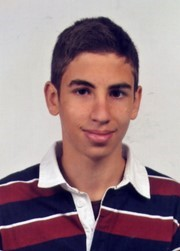
\includegraphics[height = 4cm, width=3.7cm]{capa/FranciscoMatos.jpg}\break
\end{minipage}%
\begin{minipage}{0.26\textwidth}
    Francisco Oliveira\\ \textsc{(A78416)}\\
    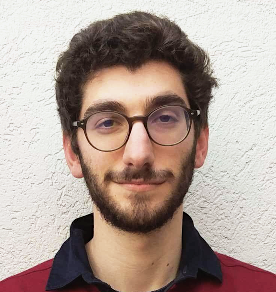
\includegraphics[height = 4cm, width=3.7cm]{capa/kiko.png}\break
\end{minipage}%
\begin{minipage}{0.26\textwidth}
    Gil Cunha\\ \textsc{(A77249)}\\
    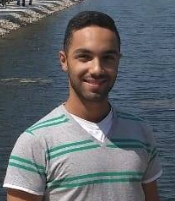
\includegraphics[height = 4cm, width=3.7cm]{capa/gil.png}\break
\end{minipage}%
\begin{minipage}{0.26\textwidth}
    Luís Costa\\ \textsc{(A74819)}\\
    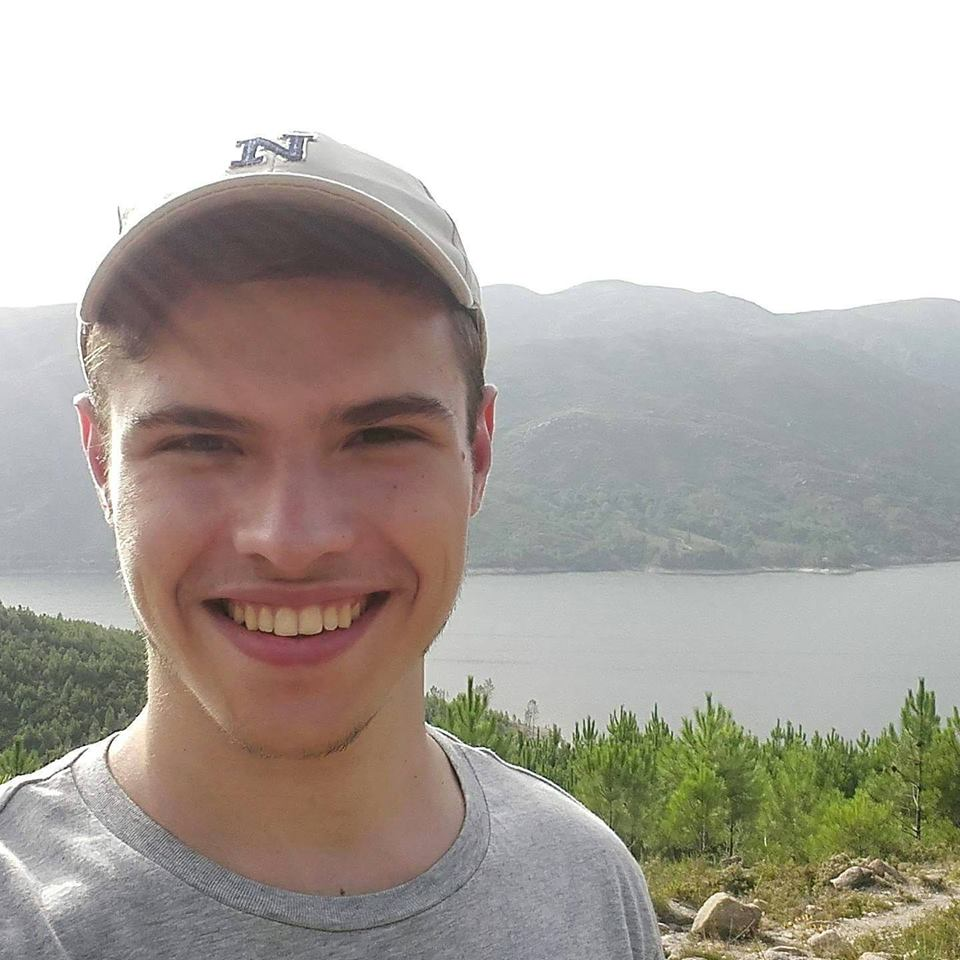
\includegraphics[height = 4cm, width=3.7cm]{capa/luis.jpg}\break
\end{minipage}%

\vfill


\end{center}
\end{titlepage}

\pagebreak
\tableofcontents
\newpage

\section{Introdução}
\hspace{3mm} 

Neste trabalho será apresentada a criação de um monitor básico para uma Base de Dados que permita a visualização, de forma simples, dos principais parâmetros de avaliação de \emph{performance} de uma BD \emph{Oracle}.

Para tal desenvolveu-se um agente em Java, que através de \emph{Views} de administração, recolhe a informação necessária e um \emph{Schema} em \emph{Oracle} para armazenamento destes mesmos dados recolhidos.

Finalmente, usando uma API em \emph{REST} ativou-se este serviço na Base de Dados (onde armazenamos os dados) e devolve-os em JSON, possibilitando uma melhor apresentação numa interface \emph{web} em HTML5.

\newpage


\section{Base de Dados}
\hspace{3mm} 

Neste trabalho prático, o grupo decidiu criar um monitor direcionado à \textbf{Base de Dados Pluggable \emph{orcl}}.
Para iniciar este projeto considerou-se importante, em primeiro lugar, a necessidade do planeamento ao nível da base de dados \emph{Oracle} a ser utilizada, antes de qualquer outra etapa. Algo a ter em conta foram os \emph{users} que teríamos de utilizar para aceder à base de dados a monitorizar, e as suas permissões. \\

Através do esquema seguinte, podemos concluir que existem vários utilizadores, com permissões diferentes entre si:

\begin{itemize}
    \item \textit{\textbf{sys.cdb:}} utilizador administrador da \emph{CDB (Container Database)}, que consegue aceder e gerir todos os seus dados gerais; 
    
    \item \textit{\textbf{sys.orcl:}} utilizador administrador da \emph{PDB (Pluggable Database)}, que consegue aceder e gerir todos os dados da PDB respetiva; 
    
    \item \textit{\textbf{hr.orcl \& grupo2.orcl:}} utilizadores comuns da \emph{PDB (Pluggable Database)}. O \textbf{grupo2} será o utilizador formado pelo grupo do projeto para criar e gerir a base de dados para o monitor final; 
\end{itemize}

\begin{figure}[H]
\centering
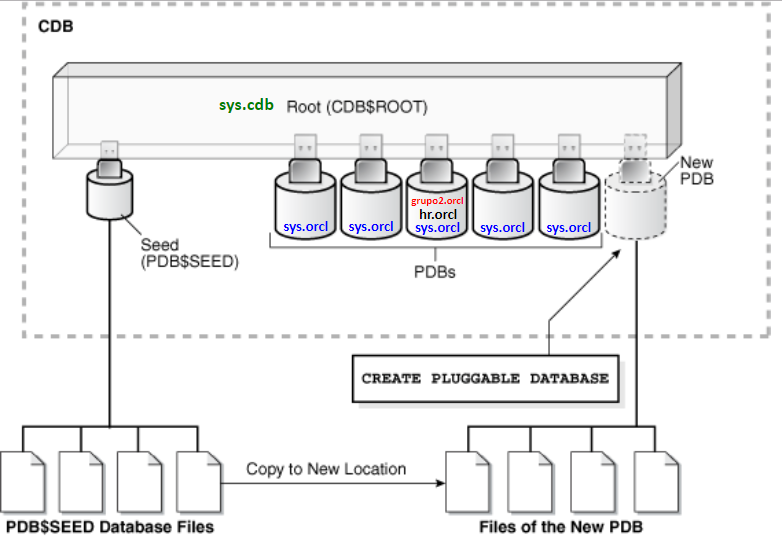
\includegraphics[scale=0.75]{arquitetura.png}
\caption{Arquitetura geral do sistema ORACLE DB}
\end{figure}

\subsection{Modelo Conceptual}
\hspace{3mm} 
O modelo conceptual desenvolvido teve por base as \emph{views} disponíveis nos utilizadores \emph{sys}, sobre a BD em questão, e as informações que o grupo considerou relevante recolher para monitorizar a base de dados. O resultado passou então numa análise prévia dos atributos das respetivas \emph{views} e da informação que estas tabelas permitiam extrair. No final, concluiu-se as seguintes entidades:
\textbf{DB, CPU, Memory, Tablespace, Datafile, User e Role.} Os respetivos atributos são explicados na secção seguinte.

O modelo conceptual desenhado apresenta-se de seguida:

\begin{figure}[H]
\centering
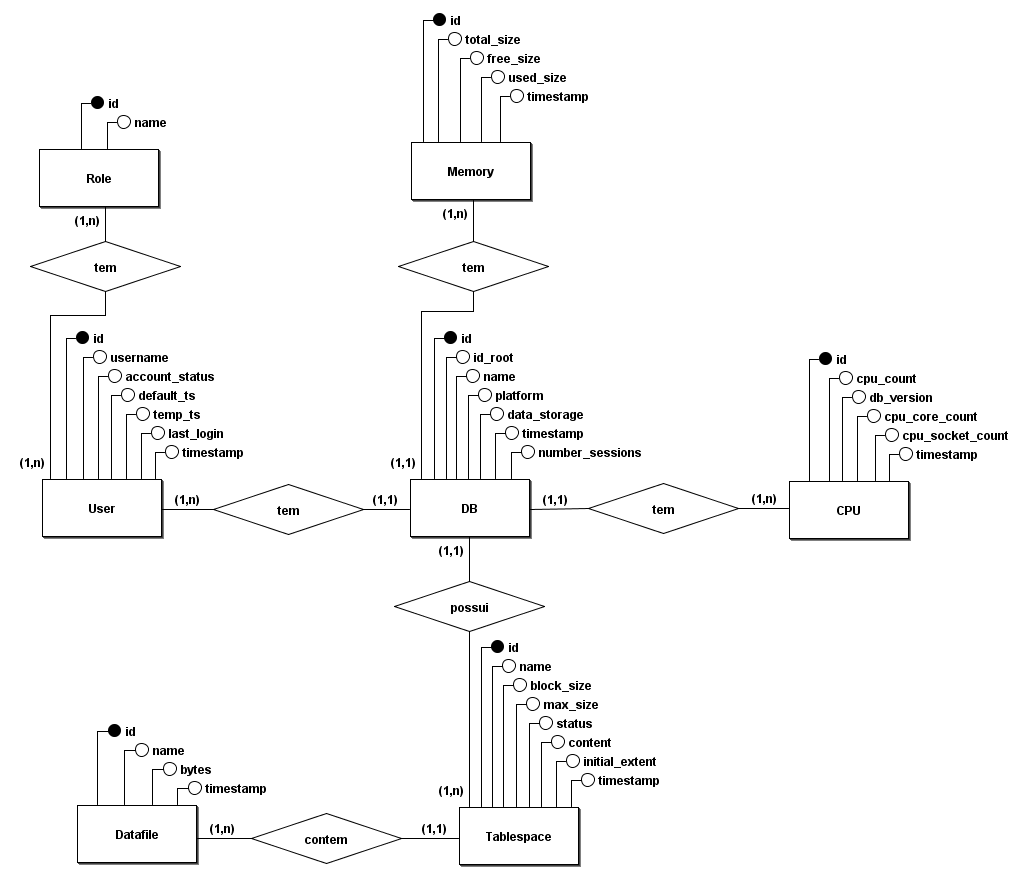
\includegraphics[scale=0.45]{modelo_conceptual.png}
\caption{Modelo Conceptual da Base de Dados do Monitor}
\end{figure}

\subsection{Análise de Entidades \& Atributos}
De forma a ter um melhor entendimento do significado das entidades e seus atributos e sobre aquilo que representam, foram geradas tabelas que os descrevem detalhadamente:\\

A entidade \textbf{DB}, referente à base de dados \emph{pluggable orcl} a analisar, possui \textbf{id\_db, id\_db\_root, name, platform, data\_storage, number\_sessions e db\_timestamp.}

\begin{figure}[H]
\centering
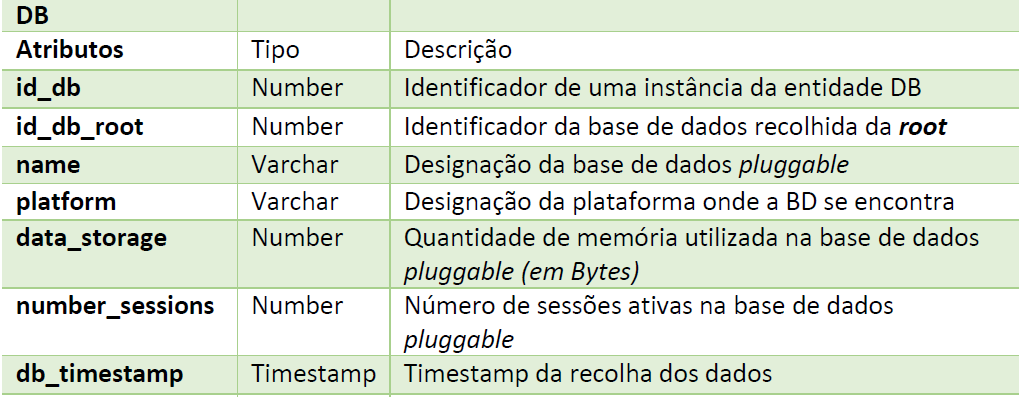
\includegraphics[scale=0.65]{db.PNG}
\caption{Informação de DB}
\end{figure}

A entidade \textbf{CPU}, referente ao cpu da base de dados \emph{Pluggable orcl}, possui \textbf{id\_cpu, db\_version, cpu\_count, cpu\_core\_count, cpu\_socket\_count e cpu\_timestamp.}

\begin{figure}[H]
\centering
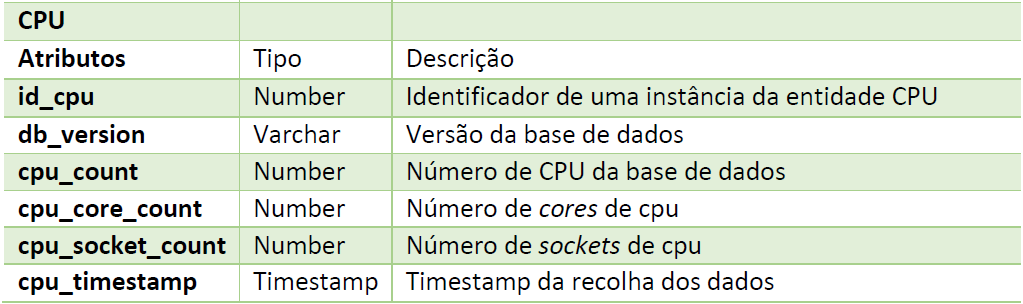
\includegraphics[scale=0.65]{cpu.PNG}
\caption{Informação de CPU}
\end{figure}

Quanto à Memória, foi necessário um estudo prévio da estrutura básica da memória da base de dados Oracle \footnote{https://docs.oracle.com/database/121/CNCPT/memory.htm#CNCPT7777}.

A base de dados Oracle possui várias áreas de memória, em que cada uma contem vários componentes. Sendo assim, o grupo focou em apenas duas das estruturas básicas da memória da BD Oracle:

\begin{itemize}
    \item \emph{\textbf{System Global Area (SGA):}} O SGA é um grupo de componentes de memória partilhada, que contêm dados e informação de controlo para uma instância da base de dados Oracle. Todos os servidores e processos em \emph{background} partilham o SGA. 
    
    \item \emph{\textbf{Program Global Area (PGA):}} O PGA é uma região de memória não partilhada que contém dados e informação de controlo exclusivamente para o uso de um processo Oracle. A base de dados Oracle cria um PGA diferente, de cada vez que um processo Oracle se inicia.
\end{itemize}

Visto estas definições, o grupo considerou mais interessante monitorizar a memória da Base de Dados \emph{Oracle}, servindo-se da informação das \emph{views} disponíveis sobre a memória, relativas ao \textbf{SGA}.\\

A entidade \textbf{Memory} possui os atributos \textbf{id\_mem, total\_size\_mb, free\_size\_mb, used\_size\_mb e mem\_timestamp.}

\begin{figure}[H]
\centering
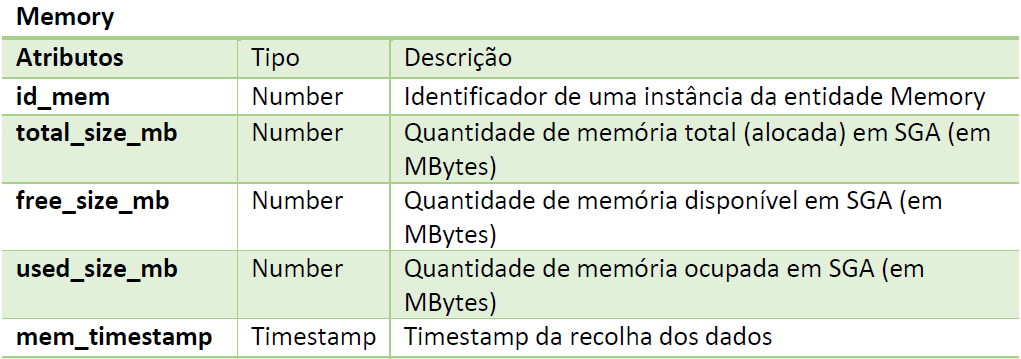
\includegraphics[scale=0.65]{memory.PNG}
\caption{Informação da Memory}
\end{figure}

A entidade \textbf{Tablespace} representa cada uma das \emph{tablespaces} associadas à BD Pluggable, e possui \textbf{id\_tablespace, name, block\_size, max\_size, status, contents, initial\_extent e ts\_timestamp.}

\begin{figure}[H]
\centering
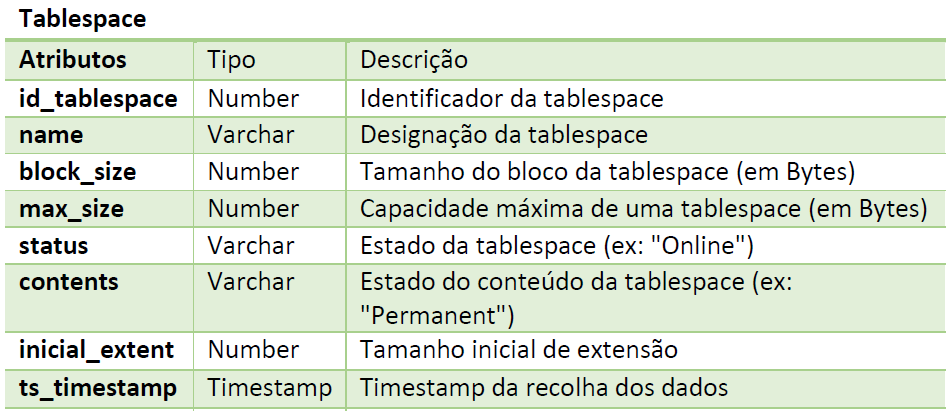
\includegraphics[scale=0.65]{tablespace.PNG}
\caption{Informação de Tablespace}
\end{figure}

A entidade \textbf{Datafile} representa cada \emph{datafile} associado a cada uma das \emph{tablespaces} que a BD Pluggable contém, e possui \textbf{id\_datafile, name, bytes e df\_timestamp}.

\begin{figure}[H]
\centering
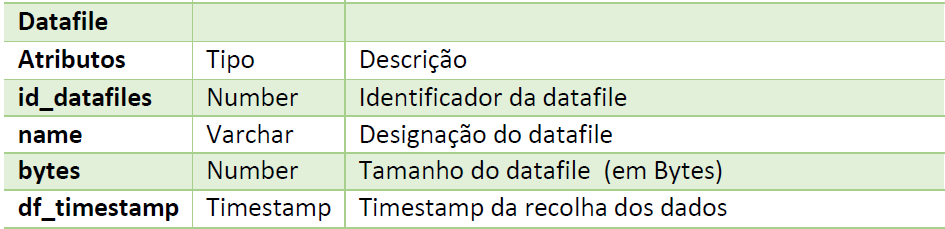
\includegraphics[scale=0.65]{datafile.PNG}
\caption{Informação de Datafile}
\end{figure}

A entidade \textbf{User} representa os utilizadores da BD Oracle e possui \textbf{id\_user, username, account\_status, default\_ts, temp\_ts, last\_login e user\_timestamp.}

\begin{figure}[H]
\centering
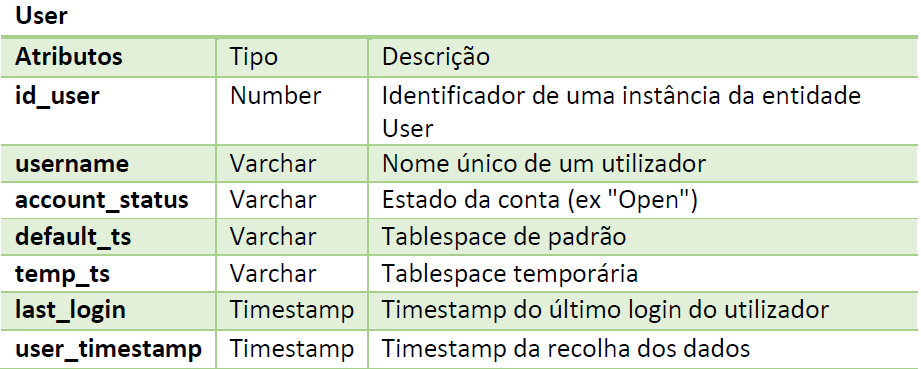
\includegraphics[scale=0.65]{user.PNG}
\caption{Informação de User}
\end{figure}

A entidade \textbf{Role} representa todos os papeis/funções (\emph{roles}) que um utilizador pode possuir na BD Oracle. Este é um conjunto de privilégios que se pode conceder a um \emph{user} e possui \textbf{id\_role e name}.

\begin{figure}[H]
\centering
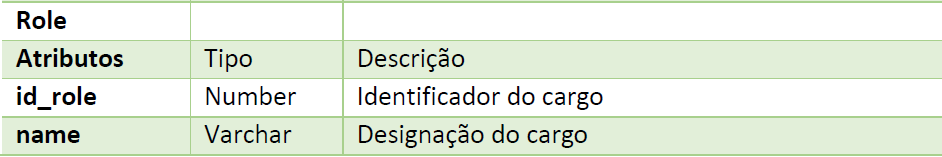
\includegraphics[scale=0.65]{role.PNG}
\caption{Informação de Role}
\end{figure}


\newpage
\subsection{Modelo Lógico}
\hspace{3mm} 

De acordo com o Modelo Conceptual foi possível proceder a realização do Modelo Lógico, tendo em especial atenção às restrições das chaves primárias e estrangeiras de cada tabela e à relação N-N presente na base de dados. O modelo lógico apresenta-se de seguida:

\begin{figure}[H]
\centering
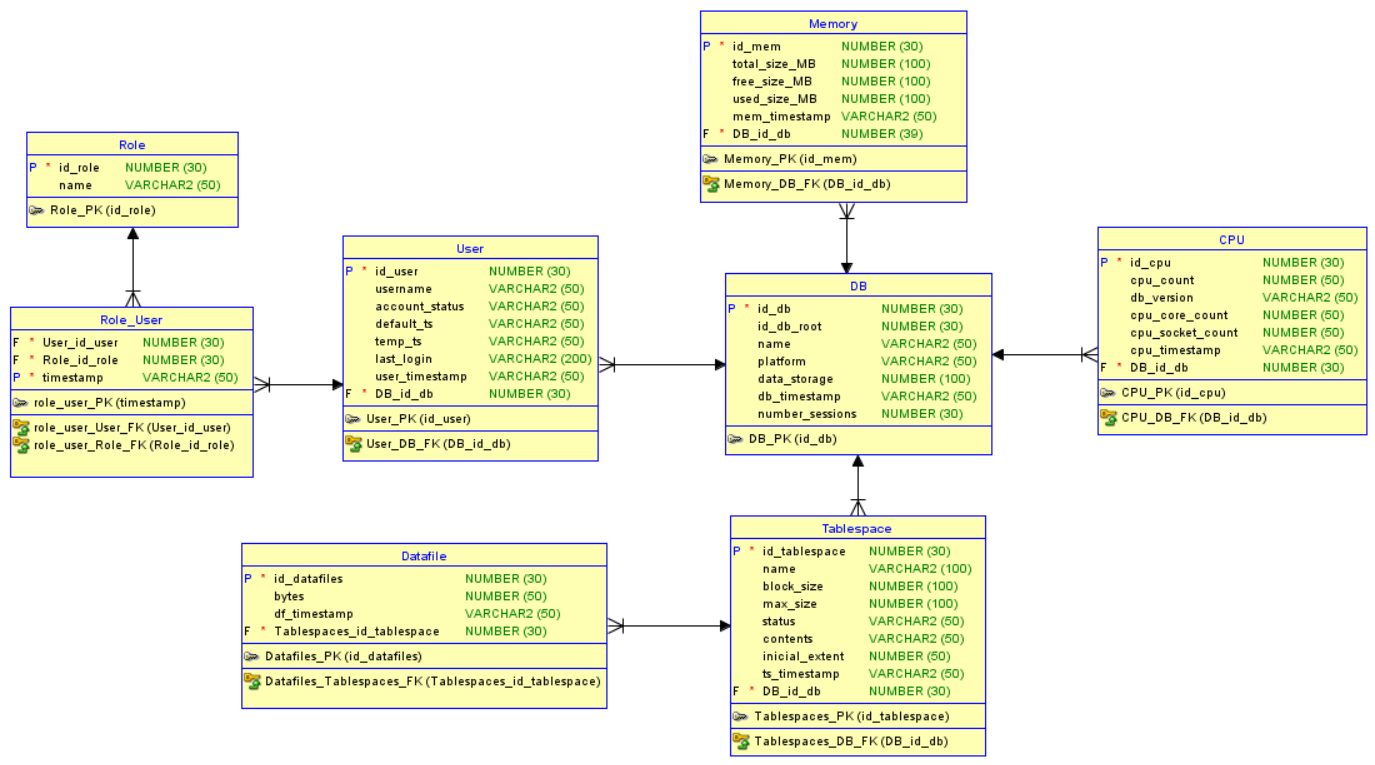
\includegraphics[scale=0.6]{modelo_logico.png}
\caption{Modelo Lógico}
\end{figure}



\subsection{Validação}
\hspace{3mm} 
De forma a validar o modelo de base de dados desenvolvido, começou-se por garantir a normalização desta. 

Com o objetivo de assegurar que este cumpra a \textbf{primeira forma normal}, foi necessário ter em atenção a relação N-N \textbf{(user-role)} no modelo lógico. Para lidar com este relacionamento, criou-se uma tabela intermediária que garantisse a atomicidade das colunas (atributos). 

Através da existência da chave primária \emph{\textbf{id}} em cada tabela, podemos garantir que todos os atributos dessa tabela estão dependentes desse mesmo \emph{id}, cumprindo assim a \textbf{segunda forma normal}. 

Por fim, visto que o nosso esquema se encontra na segunda forma normal e que nenhum atributo é dependente de um outro atributo dessa mesma tabela, exceto a chave primária, prova-se assim a \textbf{terceira forma normal} e demonstra-se que o modelo lógico se encontra normalizado.\\

Uma outra forma de validar este esquema será executando interrogações relevantes ao projeto a desenvolver. Para tal foram desenvolvidas três \emph{queries} básicas que pretendem testar o modelo lógico e a sua capacidade de resposta:
\begin{itemize}
    \item Obter o número de \emph{bytes} alocados por uma determinada base de dados;
    \item Obter o número total de \emph{tablespaces} que estão a ser monitorizadas;
    \item Obter o nome do \emph{role} de um determinado utilizador;
\end{itemize}

\hspace{2mm} 

Um pequeno esboço dessas \emph{queries} comprova a validação do esquema desenvolvido:


\begin{itemize}
    \item \texttt{SELECT total\_size\_MB FROM Memory WHERE DB\_id\_db = X};
    \item \texttt{SELECT count(id\_tablespaces) FROM tablespaces};
    \item \texttt{SELECT name FROM role INNER JOIN role\_user on role.id\_role = role\_user.Role\_id\_role WHERE User\_id\_user = X };
\end{itemize}



\subsection{Modelo Físico}
\hspace{3mm} 

\subsubsection{Criação de tabelas}

\begin{lstlisting}[ language=SQL,
                    deletekeywords={IDENTITY},
                    deletekeywords={[2]INT},
                    morekeywords={clustered},
                    framesep=8pt,
                    xleftmargin=40pt,
                    framexleftmargin=40pt,
                    frame=tb,
                    framerule=0pt ]
                    
-- TABLE DROPS
-- DROP TABLE Memory PURGE;
-- DROP TABLE CPU PURGE;
-- DROP TABLE Datafile PURGE;
-- DROP table UsersDB cascade constraints;
-- DROP TABLE Role cascade constraints;
-- DROP TABLE role_user cascade constraints;
-- DROP TABLE Tablespace PURGE;
-- DROP TABLE DB PURGE; 


-- DATABASE
CREATE TABLE db(
    id_db number(30) NOT NULL,
    id_db_root number(30) NOT NULL,
    name varchar(200) NOT NULL,
    platform varchar(20) NOT NULL,
    data_storage number(20) NOT NULL,
    number_sessions number(20) NOT NULL,
    db_timestamp varchar(50) NOT NULL,
    CONSTRAINT id_db PRIMARY KEY (id_db)
    );
    
-- MEMORY    
CREATE TABLE memory(
    id_mem          NUMBER(30) NOT NULL,
    total_size_mb   NUMBER(30),
    free_size_mb    NUMBER(30),
    used_size_mb    NUMBER(30),
    mem_timestamp   varchar(50),
    id_db_FK        NUMBER(30) NOT NULL,
    CONSTRAINT id_mem PRIMARY KEY (id_mem),
    CONSTRAINT id_db_memory
        FOREIGN KEY (id_db_FK)
        REFERENCES db(id_db)
    );
    
-- CPU
CREATE TABLE cpu(
    id_cpu number(30) NOT NULL,
    cpu_count number(20) NOT NULL,
    db_version varchar(70) NOT NULL,
    cpu_core_count number(20) NOT NULL,
    cpu_socket_count number(20) NOT NULL,
    cpu_timestamp varchar(50) NOT NULL,
    id_db_FK number(30) NOT NULL,
    CONSTRAINT id_cpu PRIMARY KEY (id_cpu),
    CONSTRAINT id_db_cpu
        FOREIGN KEY (id_db_FK)
        REFERENCES db(id_db)
    );

-- USER
CREATE TABLE usersDB(
    id_user number(30) NOT NULL,
    username varchar(70) NOT NULL,
    account_status varchar(70) NOT NULL,
    default_ts varchar(70) NOT NULL,
    temp_ts varchar(70) NOT NULL,
    last_login varchar(200) NOT NULL, 
    user_timestamp varchar(50) NOT NULL,
    id_db_FK number(30) NOT NULL,
    CONSTRAINT id_user PRIMARY KEY (id_user),
    CONSTRAINT id_db_users
        FOREIGN KEY (id_db_FK)
        REFERENCES db(id_db)
    );

-- ROLE
CREATE TABLE role(
    id_role number(30) NOT NULL,
    name varchar(70) NOT NULL,
    CONSTRAINT id_role PRIMARY KEY (id_role)
    );

-- ROLE AND USER
CREATE TABLE role_user(
    user_id_user   NUMBER(30) NOT NULL,
    role_id_role   NUMBER(30) NOT NULL,
    timestamp      VARCHAR2(50),
    CONSTRAINT role_user_user_fk 
        FOREIGN KEY ( user_id_user )
        REFERENCES usersdb ( id_user ),
    CONSTRAINT role_user_role_fk 
        FOREIGN KEY ( role_id_role )
        REFERENCES role ( id_role )
    );


-- TABLESPACE
CREATE TABLE tablespace(
    id_tablespace number(30) NOT NULL,
    name varchar(100) NOT NULL,
    block_size number(20) NOT NULL,
    max_size number(20) NOT NULL,
    status varchar(20) NOT NULL,
    contents varchar(30) NOT NULL,
    initial_extent number(20) NOT NULL,
    ts_timestamp varchar(50) NOT NULL,
    id_db_FK number(30) NOT NULL,
    CONSTRAINT id_tablespace PRIMARY KEY (id_tablespace),
    CONSTRAINT id_db_tablespace
        FOREIGN KEY (id_db_FK)
        REFERENCES db(id_db)
    );

-- DATAFILE
CREATE TABLE datafile(
    id_datafile number(30) NOT NULL,
    name varchar(150) NOT NULL,
    bytes number(20) NOT NULL,
    id_tablespace_FK numeric(20) NOT NULL,
    df_timestamp varchar(50) NOT NULL,
    CONSTRAINT id_datafile PRIMARY KEY (id_datafile),
    CONSTRAINT id_tablespace_datafile
        FOREIGN KEY (id_tablespace_FK)
        REFERENCES tablespace(id_tablespace)
    );
                    
\end{lstlisting}

\subsubsection{Sequences \& Triggers}

Visto que em Oracle SQL não é possível ter \emph{auto-increment} (como em MySQL), criou-se e utilizou-se \emph{sequences e triggers} para obter esse efeito. Assim, os ids de cada entidades serão obtidos pelas sequências e vão incrementando antes de cada inserção, através dos \emph{triggers}.

\begin{lstlisting}[ language=SQL,
                    deletekeywords={IDENTITY},
                    deletekeywords={[2]INT},
                    morekeywords={clustered},
                    framesep=8pt,
                    xleftmargin=40pt,
                    framexleftmargin=40pt,
                    frame=tb,
                    framerule=0pt ]
                    
-- SEQUENCE DROPS
-- DROP sequence db_seq;
-- DROP sequence memory_seq;
-- DROP sequence cpu_seq;
-- DROP sequence usersdb_seq;
-- DROP sequence role_seq;
-- DROP sequence tablespace_seq;
-- DROP sequence datafile_seq;

-- SEQUENCES
CREATE sequence db_seq start with 1 increment by 1 nomaxvalue;
CREATE sequence memory_seq start with 1 increment by 1 nomaxvalue;
CREATE sequence cpu_seq start with 1 increment by 1 nomaxvalue;
CREATE sequence usersdb_seq start with 1 increment by 1 nomaxvalue;
CREATE sequence role_seq start with 1 increment by 1 nomaxvalue;
CREATE sequence tablespace_seq start with 1 increment by 1 nomaxvalue;
CREATE sequence datafile_seq start with 1 increment by 1 nomaxvalue;


-- TRIGGERS
CREATE OR REPLACE TRIGGER db_trigger
BEFORE INSERT ON db
FOR EACH ROW
 WHEN (new.id_db IS NULL) 
BEGIN
  SELECT  db_seq.nextval
  INTO :new.id_db
  FROM dual;
END;
/

CREATE OR REPLACE TRIGGER memory_trigger
BEFORE INSERT ON memory
FOR EACH ROW
 WHEN (new.id_mem IS NULL) 
BEGIN
  SELECT  memory_seq.nextval
  INTO :new.id_mem
  FROM dual;
END;
/


CREATE OR REPLACE TRIGGER cpu_trigger
BEFORE INSERT ON cpu
FOR EACH ROW
 WHEN (new.id_cpu IS NULL) 
BEGIN
  SELECT  cpu_seq.nextval
  INTO :new.id_cpu
  FROM dual;
END;
/
        

CREATE OR REPLACE TRIGGER usersDB_trigger
BEFORE INSERT ON usersDB
FOR EACH ROW
 WHEN (new.id_user IS NULL) 
BEGIN
  SELECT  usersDB_seq.nextval
  INTO :new.id_user
  FROM dual;
END;
/


CREATE OR REPLACE TRIGGER role_trigger
BEFORE INSERT ON role
FOR EACH ROW
 WHEN (new.id_role IS NULL) 
BEGIN
  SELECT  role_seq.nextval
  INTO :new.id_role
  FROM dual;
END;
/  
        

CREATE OR REPLACE TRIGGER tablespace_trigger
BEFORE INSERT ON tablespace
FOR EACH ROW
 WHEN (new.id_tablespace IS NULL) 
BEGIN
  SELECT  tablespace_seq.nextval
  INTO :new.id_tablespace
  FROM dual;
END;
/  
        

CREATE OR REPLACE TRIGGER datafile_trigger
BEFORE INSERT ON datafile
FOR EACH ROW
 WHEN (new.id_datafile IS NULL) 
BEGIN
  SELECT  datafile_seq.nextval
  INTO :new.id_datafile
  FROM dual;
END;
/         

\end{lstlisting}



\subsection{Utilizador}
\hspace{3mm} 
De forma a ser possível obter a informação necessária para preencher a base de dados, será necessário aceder a diversas \emph{views}, para tal serão precisos \emph{users} que tenham acessos a estas. O \emph{user} que tipicamente tem esse acesso é o \emph{sys}, e visto que se pretende recolher não só informação da \emph{plugable DB} como também da \emph{root DB}, serão necessários.
Por fim, um terceiro utilizador, \emph{grupo2}, foi criado, onde será gerado o modelo físico da base de dados que guardará as informações relevantes para o projeto.

\begin{lstlisting}[ language=SQL,
                    deletekeywords={IDENTITY},
                    deletekeywords={[2]INT},
                    morekeywords={clustered},
                    framesep=8pt,
                    xleftmargin=40pt,
                    framexleftmargin=40pt,
                    frame=tb,
                    framerule=0pt ]
                    
-- USER grupo2
CREATE USER grupo2 IDENTIFIED BY pass  
DEFAULT TABLESPACE TP_AEBD
TEMPORARY TABLESPACE TP_TEMP
PASSWORD EXPIRE ;

ALTER USER grupo2 QUOTA UNLIMITED ON TP_AEBD;

-- GRANTS to grupo2
GRANT "DBA" TO grupo2 ;

GRANT CREATE SESSION TO grupo2 ;
GRANT CREATE TABLE TO grupo2 ;

-- TEST CONNECTION
connect grupo2/pass;

show user;  
                    
\end{lstlisting}


\subsubsection{Tablespaces \& Datafiles associados}
\hspace{3mm}

\begin{lstlisting}[ language=SQL,
                    deletekeywords={IDENTITY},
                    deletekeywords={[2]INT},
                    morekeywords={clustered},
                    framesep=8pt,
                    xleftmargin=40pt,
                    framexleftmargin=40pt,
                    frame=tb,
                    framerule=0pt ]

-- TABLESPACE TP_AEBD
CREATE TABLESPACE TP_AEBD 
    DATAFILE 
        '\u01\app\oracle\oradata\orcl12\orcl\TP_AEBD_01.DBF' SIZE 104857600;

-- TABLESPACE TP_TEMP   
CREATE TEMPORARY TABLESPACE TP_TEMP 
    TEMPFILE 
        '\u01\app\oracle\oradata\orcl12\orcl\TP_TEMPORARY_01.DBF' SIZE 52428800 AUTOEXTEND ON NEXT 104857600 MAXSIZE 34359721984 
    EXTENT MANAGEMENT LOCAL UNIFORM SIZE 1048576;                    
                    
\end{lstlisting}

\section{Ligação à Base de Dados}
\hspace{3mm} 

DO ME NEXT PLS :C

sys.cdb -> select memory e cpu
sys.orcl -> select o resto
grupo2.orcl -> insert de tudo

\section{Agente de Recolha de Informação}
\hspace{3mm} 

O Agente de Recolha de Informação foi desenvolvido em \emph{Java}. Este apresenta as seguintes classes:
\begin{itemize}
    \item BDConnection
    \item Selects
    \item Inserts
    \item Main
\end{itemize}

\subsection{Classes}
\hspace{3mm} 

\subsubsection{BDConnection}
\hspace{3mm} 

Esta classe estabelece a ligação à Base de Dados através dos diferentes utilizadores. Utiliza o utilizador \emph{sys}, tanto para a \emph{plugable} DB como para a \emph{Root} DB, visto que será necessário aceder a ambas, para obter informação especifica. 
Também é estabelecida a conexão a um utilizador pertencente à \emph{plugable} DB, \emph{grupo2}, que possui acesso à Base de Dados que irá guardar toda a informação recolhida.

\subsubsection{Selects}
\hspace{3mm} 

Esta classe é responsável pela recolha de informação relativamente aos parâmetros de avaliação da \emph{performance} da Base de Dados \emph{Oracle}, definidos pelo grupo. Sendo assim, esta classe verifica qual a informação a obter, liga-se ao utilizador \emph{sys} da \emph{root} ou da \emph{plugable} DB de acordo com o parâmetro desejado e, através de um \emph{SELECT} simples, seleciona/recolhe esses dados.

\subsubsection{Inserts}
\hspace{3mm} 

Por sua vez, a classe \emph{Inserts} gere a inserção de dados na Base de Dados. Para tal, utiliza a conexão referente ao utilizador \emph{Grupo2}, previamente criado, e executa um \emph{INSERT} simples, a partir dos dados obtidos através das \emph{views} na classe \emph{Selects}. É assim realizado o armazenamento dos dados sobre a \emph{performance} da Base de Dados em questão. 

\subsubsection{Main}
\hspace{3mm} 

Esta classe é responsável pelo inicío de todo o processo de recolha e armazenamento de dados.\\

\subsection{API REST}
\hspace{3mm} 

Os \emph{\textbf{Oracle REST Data Services (ORDS)}} permitem desenvolver interfaces \emph{REST} para Bases de Dados Oracle relacionais. Foi através destes serviços, incorporados na aplicação SQL Developer, que nos era fornecida a opção de inicialização de um serviço REST, pelo que se decidiu utilizar esta alternativa, de modo a facilitar e agilizar o processo.

\subsubsection{Ativação dos serviços REST para a BD}
\hspace{3mm} 

Em primeiro lugar, houve a necessidade de ativar os  \emph{\textbf{REST services}} para a ligação do nosso utilizador à Base de Dados -  \emph{\textbf{grupo2.orcl}}. Para isso, bastou ir à opção "REST Services" de \emph{\textbf{grupo2.orcl}}, onde ativamos os serviços REST em "Enable REST Services...", visível na imagem abaixo:

\begin{figure}[H]
\centering
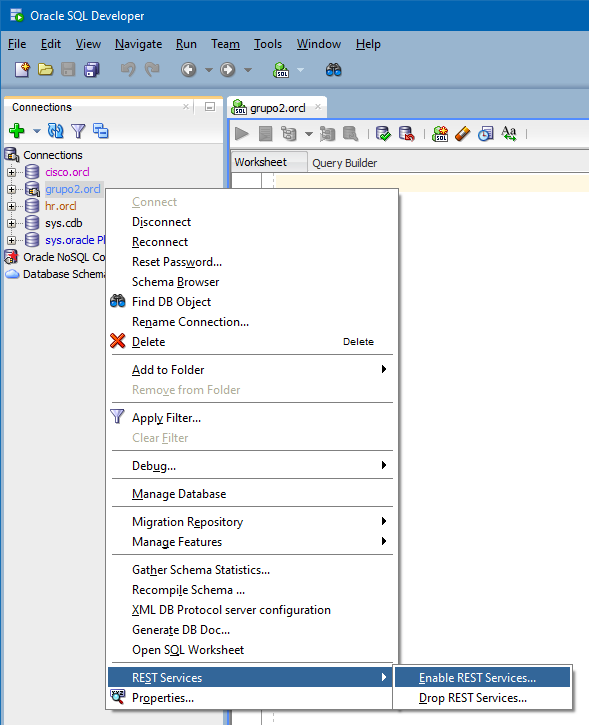
\includegraphics[scale=0.55]{REST/rest_grupo2_1.png}
\caption{Ativação dos serviços REST em grupo2.orcl}
\end{figure}

De seguida é nos apresentado o \emph{wizard} de configuração.
Na primeira janela \textbf{(figura 11)} marcamos a caixa \emph{"Enable schema"} e definimos o \emph{"Schema alias"} como \textbf{grupo2}. Este nome será necessário mais tarde nos pedidos \emph{web}. Se fosse pretendido uma maior segurança, seria possível mudar o \emph{alias} para algo diferente do nome original, bem como marcar a última caixa para ativar autenticação nos pedidos. No entanto, esta situação não foi considerada relevante para este trabalho.

\begin{figure}[H]
\centering
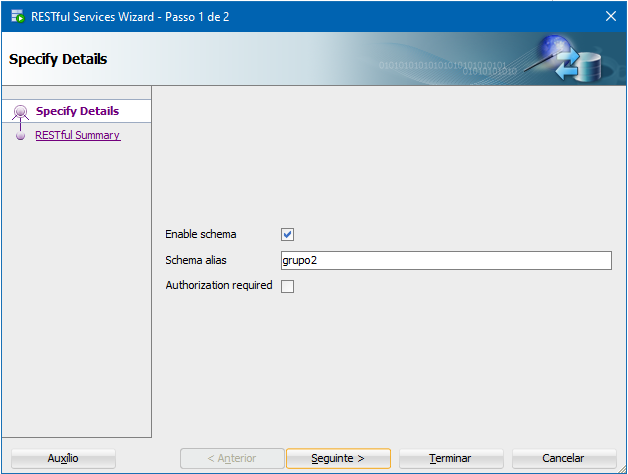
\includegraphics[scale=0.6]{REST/rest_grupo2_2.png}
\caption{Ativação dos serviços REST - Wizard}
\end{figure}

Nesta segunda janela, permite a confirmação das opções selecionadas préviamente e finaliza-se a configuração:

\begin{figure}[H]
\centering
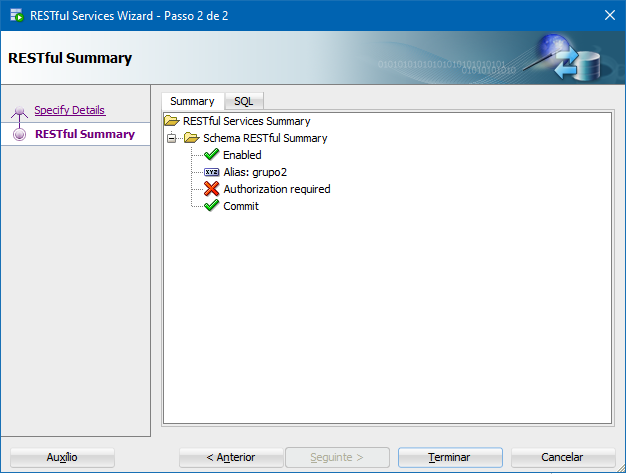
\includegraphics[scale=0.6]{REST/rest_grupo2_3.png}
\caption{Ativação dos serviços REST - Wizard}
\end{figure}

\subsubsection{Ativação das tabelas}
\hspace{3mm} 

Depois de ativar o \emph{REST service} na nossa ligação -- \emph{\textbf{grupo2.orcl}} : utilizador e BD --  falta ainda ativá-lo para todas as tabelas que pretendemos ter acesso \emph{via REST}, ou seja, todas as tabelas da nossa BD.
Segue-se um exemplo para a tabela CPU. O processo é o mesmo, nas opções da tabela selecionamos \emph{"Enable REST Services..."}, de forma a abrir o \emph{wizard}, como na imagem abaixo.

\begin{figure}[H]
\centering
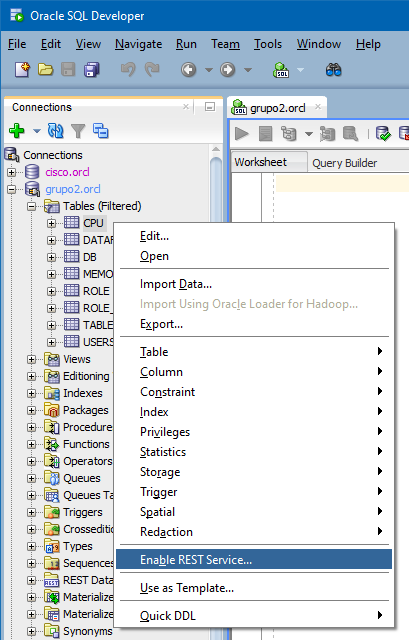
\includegraphics[scale=0.6]{REST/rest_tabela_1.png}
\caption{Ativação dos serviços REST na tabela CPU}
\end{figure}

Já no \emph{wizard} o processo é exatamente igual ao de ativação para a BD, apenas sendo necessário referir que todas as tabelas mantiveram um \emph{alias} igual ao nome da tabela, com exceção da tabela \textbf{USERSDB} que foi nomeado de \textbf{user} e da tabela  \emph{\textbf{ROLE\_USER}} que não foi ativada.\\

\subsubsection{API}
\hspace{3mm} 

TODO gil pls upgrade o look desta subsubsection

Como a interface REST foi gerada automaticamente pelo ORDS a nossa API será a que foi gerada. Esta API mostrouse muito prática e simples de usar.

Qualquer pedido GET retorna um JSON com a informação pretendida.
Os pedidos seguem a seguinte formula:

http://localhost:8080/ords/{alias da DB}/{alias da tabela}/
\newline (alguem pode melhorar o look da formula pls? )

onde substituímos apenas os "alias da DB" e "tabela" pelos nomes das que pretendemos aceder.

Temos aqui como exemplo um pedido à DB "grupo2" e tabela "db":

\begin{figure}[H]
\centering
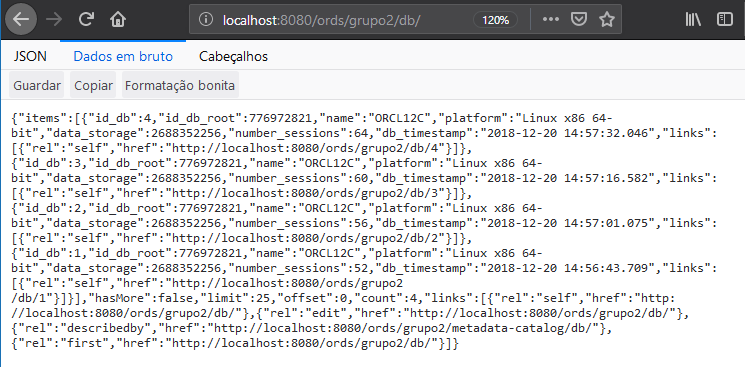
\includegraphics[scale=0.75]{REST/api_1.png}
\caption{Exemplo de um pedido GET ao grupo2:db}
\end{figure}

Podemos também efetuar GETS mais precisos, adicionando condições á query.
Segue a imagem de um exemplo onde efetuamos o pedido anterior mas onde apenas queriamos a entrada com "id\_db" igual a 1.

\begin{figure}[H]
\centering
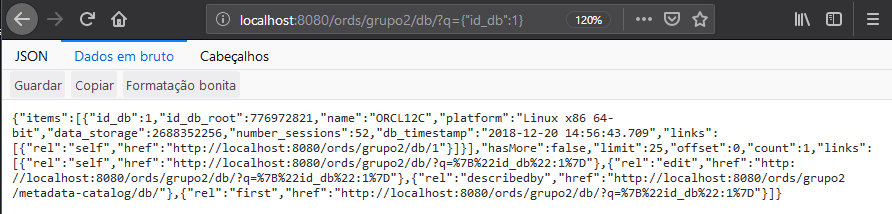
\includegraphics[scale=0.6]{REST/api_2.png}
\caption{Exemplo de um pedido GET ao grupo2:db}
\end{figure}

A API gerada permite também pedidos de POST, PUT, DELETE, entre outros, contudo estes não se mostrar necessários para o nosso trabalho.


\section{Interface Web}
\hspace{3mm} 

Na interface web preparamos uma Homepage com informação sobre o trabalho e uma página individual para cada tabela que pretendíamos visualizar.



\subsection{Screenshots}
\hspace{3mm} 
USAR SWINGBENCH PARA CRIAR CARGA NA BASE DE DADOS (FICHA 6)



%\begin{figure}[H]
%\centering
%\includegraphics[scale=0.5]{142.png}
%\caption{Exercicio 15}
%\end{figure}

\newpage
\section{Conclusão}
\hspace{3mm} 

\end{document}